%% Copyright (c) 2015-2019, RTE (http://www.rte-france.com)
%% See AUTHORS.txt
%% All rights reserved.
%% This Source Code Form is subject to the terms of the Mozilla Public
%% License, v. 2.0. If a copy of the MPL was not distributed with this
%% file, you can obtain one at http://mozilla.org/MPL/2.0/.
%% SPDX-License-Identifier: MPL-2.0
%%
%% This file is part of Dynawo, an hybrid C++/Modelica open source time domain simulation tool for power systems.

\documentclass[a4paper, 12pt]{report}

%% Except where otherwise noted, content in this documentation is Copyright (c)
%% 2015-2019, RTE (http://www.rte-france.com) and licensed under a
%% CC-BY-4.0 (https://creativecommons.org/licenses/by/4.0/)
%% license. All rights reserved.

% Latin Modern fam­ily of fonts
\usepackage{lmodern}

\usepackage[english]{babel}

% specify encoding
\usepackage[utf8]{inputenc} % input
\usepackage[T1]{fontenc} % output

% Document structure setup
\usepackage{titlesec} % To change chapter format
\setcounter{tocdepth}{3} % Add subsubsection in Content
\setcounter{secnumdepth}{3} % Add numbering for subsubsection
\setlength{\parindent}{0pt} % No paragraph indentation

% Change title format for chapter
\titleformat{\chapter}{\Huge\bf}{\thechapter}{20pt}{\Huge\bf}

% To add links on page number in Content and hide red rectangle on links
\usepackage[hidelinks, linktoc=all]{hyperref}
\usepackage[nottoc]{tocbibind}  % To add biblio in table of content
\usepackage{textcomp} % For single quote
\usepackage{url} % Allow linebreaks in \url command
\usepackage{listings} % To add code samples

% Default listings parameters
\lstset
{
  aboveskip={1\baselineskip}, % a bit of space above
  backgroundcolor=\color{shadecolor}, % choose the background color
  basicstyle={\ttfamily\footnotesize}, % use font and smaller size \small \footnotesize
  breakatwhitespace=true, % sets if automatic breaks should only happen at whitespace
  breaklines=true, % sets automatic line breaking
  columns=fixed, % nice spacing -> fixed / flexible
  mathescape=false, % escape to latex false
  numbers=left, % where to put the line-numbers
  numberstyle=\tiny\color{gray}, % the style that is used for the line-numbers
  showstringspaces=false, % do not emphasize spaces in strings
  tabsize=4, % number of spaces of a TAB
  texcl=false, % activates or deactivates LaTeX comment lines
  upquote=true % upright quotes
}

% Avoid numbering starting at each chapter for figures
\usepackage{chngcntr}
\counterwithout{figure}{chapter}

\usepackage{tikz} % macro pack­age for cre­at­ing graph­ics
\usepackage{pgfplots} % draws func­tion plots (based on pgf/tikz)

\usepackage{algorithm} % Add algorithms
\usepackage[noend]{algpseudocode} %  all end ... lines are omitted in algos

\usepackage{amsmath} % Add math­e­mat­i­cal fea­tures
\usepackage{schemabloc} % Add block diagram library (french one)

\usepackage{adjustbox} % Add box for flowchart

\usepackage{booktabs} % for toprule and midrule in tables

\usepackage{tabularx}

\usepackage[nolist]{acronym} % don’t write the list of acronyms.
% Acronyms list
\begin{acronym}
\acro{BDF}{Backward Differentiation Formula}
\acro{BE}{Backward Euler}
\acro{DAE}{Differential Algebraic Equations}
\acro{IDA}{Implicit Differential-Algebraic solver}
\acro{LLNL}{Lawrence Livermore National Lab}
\acro{KINSOL}{Krylov Inexact Newton SOLver}
\acro{NR}{Newton-Raphson}
\acro{PLL}{Phase-Locked Loop}
\acro{SVC}{Static Var Compensator}
\acro{SUNDIALS}{SUite of Nonlinear and DIfferential/ALgebraic equation Solvers}
\acro{WECC}{Western Electricity Coordinating Council}
\end{acronym}

% Syntax highlight
%% Except where otherwise noted, content in this documentation is Copyright (c)
%% 2015-2019, RTE (http://www.rte-france.com) and licensed under a
%% CC-BY-4.0 (https://creativecommons.org/licenses/by/4.0/)
%% license. All rights reserved.

\usepackage{color}

\definecolor{blue}{rgb}{0,0,1}
\definecolor{lightblue}{rgb}{.3,.5,1}
\definecolor{darkblue}{rgb}{0,0,.4}
\definecolor{red}{rgb}{1,0,0}
\definecolor{darkred}{rgb}{.56,0,0}
\definecolor{pink}{rgb}{.933,0,.933}
\definecolor{purple}{rgb}{0.58,0,0.82}
\definecolor{green}{rgb}{0.133,0.545,0.133}
\definecolor{darkgreen}{rgb}{0,.4,0}
\definecolor{gray}{rgb}{.3,.3,.3}
\definecolor{darkgray}{rgb}{.2,.2,.2}
\definecolor{shadecolor}{gray}{0.925}

% **********************************************************************************
% Syntax : Bash (bash)
% **********************************************************************************

\lstdefinelanguage{bash}
{
  keywordstyle=\color{blue},
  morekeywords={
    cd,
    export,
    source},
  numbers=none,
  deletekeywords={jobs}
}

% **********************************************************************************
% Syntax : XML
% **********************************************************************************

\lstdefinelanguage{XML}
{
  morestring=[s][\color{purple}]{"}{"},
  morecomment=[s][\color{green}]{<?}{?>},
  morecomment=[s][\color{green}]{<!--}{-->},
  stringstyle=\color{black},
  identifierstyle=\color{blue},
  keywordstyle=\color{red},
  morekeywords={
    xmlns,
    xsi,
    noNamespaceSchemaLocation,
    type,
    source,
    target,
    version,
    tool,
    transRef,
    roleRef,
    objective,
    eventually}
}

% **********************************************************************************
% Syntax : Modelica (modelica)
% **********************************************************************************
\lstdefinelanguage{Modelica}{
  alsoletter={...},
  morekeywords=[1]{ % types
      Boolean,
      Integer,
      Real},
  keywordstyle=[1]\color{red},
  morekeywords=[2]{ % keywords
    algorithm,
    and,
    annotation,
    assert,
    block,
    class,
    connector,
    constant,
    discrete,
    else,
    elseif,
    elsewhen,
    end,
    equation,
    exit,
    extends,
    external,
    false,
    final,
    flow,
    for,
    function,
    if,
    in,
    inner,
    input,
    import,
    loop,
    model,
    nondiscrete,
    not,
    or,
    outer,
    output,
    package,
    parameter,
    public,
    protected,
    record,
    redeclare,
    replaceable,
    return,
    size,
    terminate,
    then,
    true,
    type,
    when,
    while},
  keywordstyle=[2]\color{darkred},
  morekeywords=[3]{ % functions
    abs,
    acos,
    asin,
    atan,
    atan2,
    Complex,
    connect,
    conj,
    cos,
    cosh,
    cross,
    der,
    edge,
    exp,
    fromPolar,
    imag,
    noEvent,
    pre,
    sign,
    sin,
    sinh,
    sqrt,
    tan,
    tanh},
  keywordstyle=[3]\color{blue},
  morecomment=[l][\color{green}]{//}, % comments
  morecomment=[s][\color{green}]{/*}{*/}, % comments
  morestring=[b][\color{pink}]{'}, % strings
  morestring=[b][\color{pink}]{"}, % strings
}


\usepackage{xspace} % Define typography
\usepackage{dirtree}
\newcommand{\Dynawo}[0]{Dyna$\omega$o\xspace}


\begin{document}

\chapter{IEEE14}

The IEEE 14-bus system is a standard test case in the power system community. It represents a simple approximation of the American Electric Power system (in the U.S. Midwest) as it was in the early 1960s. The data were provided by Iraj Dabbagchi of AEP and converted into the IEEE Common Data Format by Rich Christie at the University of Washington in August 1993.

% Generic description of the non regression test
% List of scenarios
\section{Test case description}

The IEEE 14-bus test case system has 14 buses, 5 generators (three of them being synchronous compensators used only for reactive support), 1 shunt, 3 transformers, 16 lines and 11 loads.\\
There are two voltage levels in the test case: 69 kV and 13.8 kV. The lower part of the system, with generators 1, 2 and 3, corresponds to the 69 kV network, whereas the upper part is the 13.8 kV network.

\begin{figure}[H]
  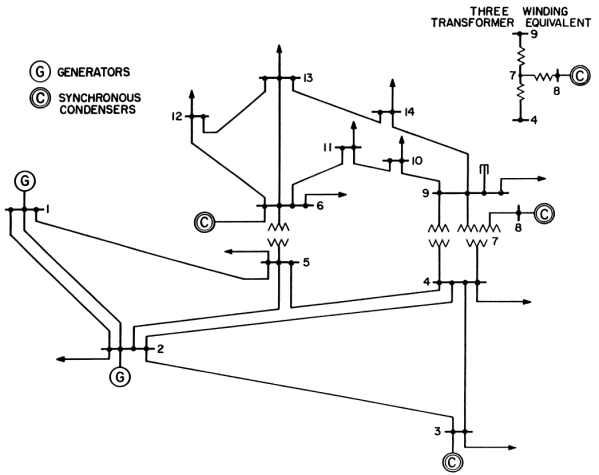
\includegraphics[width=\textwidth]{Single-line-diagram-of-IEEE-14-bus-system.png}
  \caption{IEEE 14 bus system diagram}
\end{figure}

\subsection{Initial Conditions}

The reference angle for the load flow is set at bus n°1. \\

Here are the initial conditions for each generator.

\begin{center}
\begin{tabular}{|c|c|c|c|c|}
  \hline
  Generator & P (MW) & Q (Mvar) & U (kV) & $\Theta$ (°) \\
  \hline
  1 & 232.39 & -16.55 & 73.14 & 0.00\\
  2 & 40.00 & 43.56 & 72.11 & -4.98\\
  3 & 0.00 & 25.07 & 69.69 & -12.73\\
  6 & 0.00 & 12.73 & 14.77 & -14.22\\
  8 & 0.00 & 17.62 & 15.04 & -13.36\\
  \hline
\end{tabular}
\end{center}

\subsection{Models}

\subsubsection{Synchronous Machines}

The generators are modelled using the GeneratorPVSignalN model. This model is used for the calculation of steady states after an event. All machines participate in the frequency regulation depending on their active power setpoint (although the frequency is not explicitly modelled in this model). All machines regulate the voltage at their stator.

All parameters can be found in the IEEE14.par file.

\subsubsection{System reference frequency handling}

The model used for frequency handling is DYNModelSignalN. It calculates the power compensation needed to stabilize the system at each time step. This compensation is instantaneous.

\subsubsection{Loads}

Loads follow an alpha beta dynamic behaviour, with a load restoration when the voltage is between UMinPu and UMaxPU.

They are directly connected to the grid (no transformer included).


\subsection{Scenarios}
The simulated scenario is a disconnection of line 1-5.

\subsection{Solver}
The solver used is the simplified solver SIM with hMin = 1 and hMax = 10.


\newpage
\section{Results}

For each event, we focus on generator 1 's response.

At $t=1s$, the line between buses 1 and 5 is opened at its bus 5 's extremity. 75.6 W and 3.1 Mvar of active and reactive power are initially transiting on this line (from bus 1 to bus 5).\\
One can observe that the generator active power adapts to compensate the desequilibrium. The dynamics are linked to the load restoration dynamics.

\begin{figure}[H]
\subfigure[Active power (MW)]
{%
  \begin{tikzpicture}
    \begin{axis}[height = 2in]
        \addplot[color=blue!50]
        table[x=time, y=GEN____1_SM_generator_PGenPu]
        {../reference/outputs/curves/curves.csv};
    \end{axis}
  \end{tikzpicture}
}
\subfigure[Reactive power (Mvar)]
{%
  \begin{tikzpicture}
    \begin{axis}[height = 2in]
        \addplot[color=blue!50]
        table[x=time, y=GEN____1_SM_generator_QGenPu]
        {../reference/outputs/curves/curves.csv};
    \end{axis}
  \end{tikzpicture}
}
\caption{Generator 1 response to the disconnection}
\end{figure}


\end{document}
